% paper/sections/12u10_common_flux_ledger.tex
%
% U10: Conservative common-flux ledger gate — Tier VIII
% ═══════════════════════════════════════════════════════════════════════════════
\subsubsection{U10：保存形共通フラックス台帳 [Tier VIII]}
\label{sec:U10_common_flux_ledger}

\paragraph{検証対象．}
保存形共通フラックス経路では，CLS 変数 $\psi$ だけでなく，
アフィン密度 $\rho(\psi)$ と運動量 $\rho\bu$ も同じ FCCD 面フラックス台帳で更新される
必要がある（§\ref{sec:cls_advection}, §\ref{sec:algorithm}）．
U10 は，この台帳同一性を component level で検証する．
体積だけを後から合わせる，または $\psi$ だけを clip/project する経路は，
密度・運動量に同じ保存写像を与えないため合格経路とはしない．

\paragraph{設定．}
周期正方領域上の滑らかな $\psi$ を FCCD flux-form + TVD-RK3 で 1 step 更新し，
返された stage ledger を \texttt{ConservativeCommonFluxTransport} へ渡す．
密度は
\[
  \rho(\psi)=\rho_g+(\rho_l-\rho_g)\psi
\]
とし，$\rho_l/\rho_g\in\{1,10,100,833.333\}$，
$N\in\{32,64,128\}$，CFL $\in\{0.10,0.30,0.60\}$ を調べる．
正の候補は一様速度場に対する共通台帳更新であり，
負対照は (i) 非アフィン密度，(ii) $\psi$ だけを射影した ledger である．

\paragraph{結果．}

\begin{table}[!ht]
\caption{U10：保存形共通フラックス台帳 gate}
\label{tab:U10_common_flux_ledger}
\PaperCaptionNote{全 $N$，密度比，CFL の組合せで closed candidate は密度・運動量保存とアフィン密度写像を満たし，負対照 2 件は fail-closed した．周期格子の保存量は重複 endpoint を除く unique tensor grid 上で測る．}
\centering\small
\begin{tabular}{l c}
\toprule
指標 & 実測値 \\
\midrule
最大相対エネルギー増分 $\max(\Delta K/K_0)$ & $0.000\times10^{0}$ \\
最大密度積分誤差 $\max|\Delta M_\rho|$ & $1.137\times10^{-13}$ \\
最大運動量積分誤差 $\max|\Delta P_i|$ & $2.842\times10^{-14}$ \\
最大アフィン密度誤差 & $0.000\times10^{0}$ \\
負対照 reject & $2/2$ \\
\bottomrule
\end{tabular}
\end{table}

\begin{figure}[!ht]
\centering
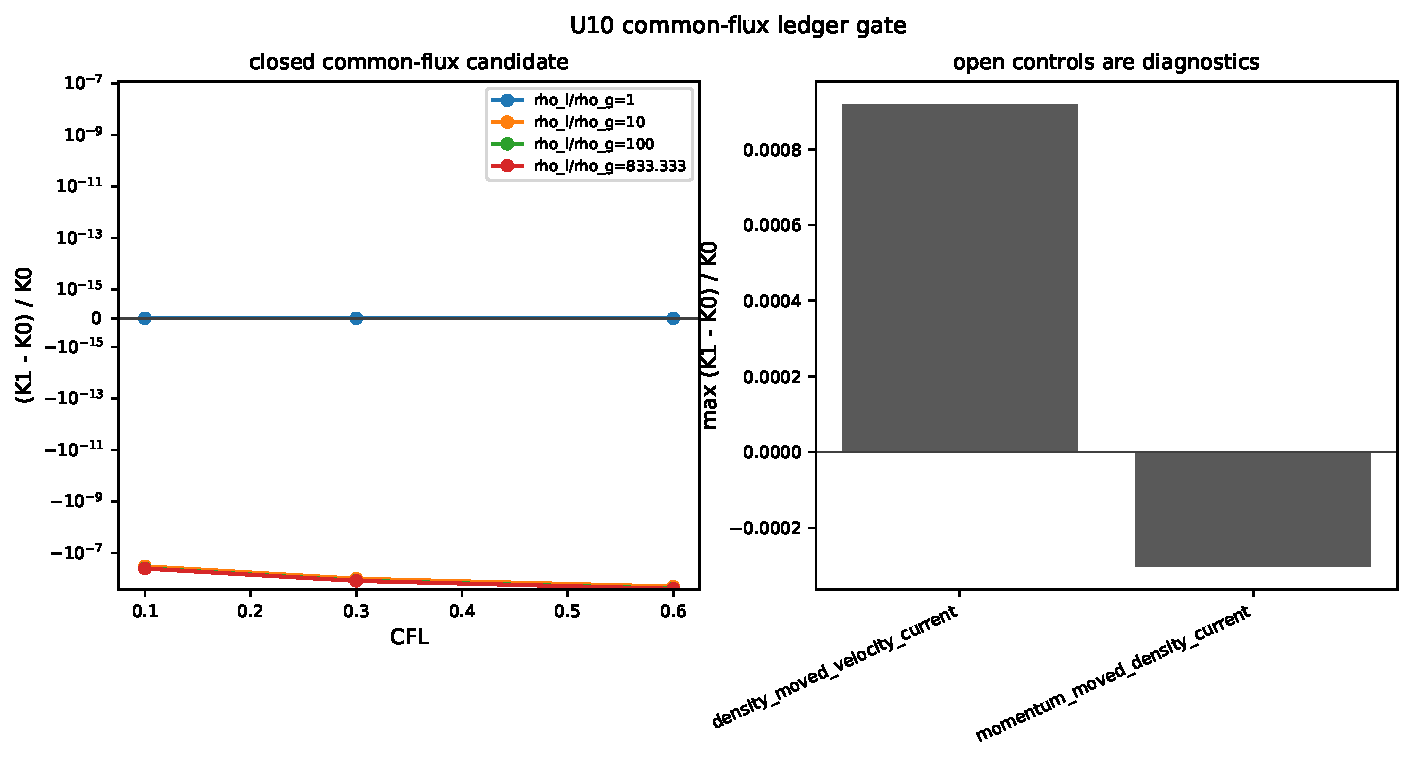
\includegraphics[width=0.92\linewidth]{figures/ch12_u10_common_flux_ledger}
\caption{U10：保存形共通フラックス台帳 gate}
\label{fig:ch12_u10_common_flux_ledger}
\PaperCaptionNote{左：closed common-flux candidate の相対エネルギー増分は全 CFL・密度比で非正．右：密度を先に動かして速度を据え置く，または運動量だけを別写像で動かす open control は診断値として分離し，保存形共通フラックスの合格経路へは入れない．}
\end{figure}

\paragraph{判定と次章への接続．}
U10 は \checkmark と判定する．
これは保存形共通フラックス経路の component gate であり，
第13章の V 系列へ新しい物理 benchmark として追加するものではない．
共通フラックスを用いる実際の有限振幅二相流応答は，第~\ref{sec:benchmarks}章の
canonical 物理 benchmark で扱う．

\FloatBarrier
